% =============================================================================
% RGS-Halso Business Plan – Comprehensive Lesotho-Focused Version (2026)
% Author: Zwelihle Mathe (DJ Zwesta SA)
% Last major update: February 2026
% Compile: xelatex --shell-escape RGS_Halso_BusinessPlan_Combined.tex
% =============================================================================

\documentclass[11pt,a4paper]{article}

\usepackage{fontspec}
\setmainfont{Times New Roman}

\usepackage{geometry}
\geometry{left=20mm,right=20mm,top=20mm,bottom=25mm}

\usepackage{longtable,booktabs,multirow,array,tabularx}
\usepackage{graphicx}
\usepackage{xcolor}
\definecolor{rgsblue}{RGB}{0,51,102}
\definecolor{rgsgreen}{RGB}{0,153,76}
\definecolor{rgsorange}{RGB}{255,140,0}

\usepackage{hyperref}
\hypersetup{colorlinks=true, linkcolor=rgsblue, urlcolor=rgsgreen}

\usepackage{fancyhdr}
\pagestyle{fancy}
\fancyhf{}
\fancyhead[L]{\textcolor{rgsblue}{\textbf{RGS Construction Lesotho (Pty) Ltd}}}
\fancyhead[R]{\textcolor{rgsgreen}{Lesotho ECO Homes \& Halso Gas Partnership}}
\fancyfoot[L]{\small Zwelihle Mathe (DJ Zwesta SA) \quad $|$ \quad +27 65 926 9311 \quad $|$ \quad zwexman@gmail.com}
\fancyfoot[C]{\small \thepage}
\fancyfoot[R]{\small \textcolor{red}{Confidential}}
\renewcommand{\headrulewidth}{0.4pt}
\setlength{\headheight}{15pt}

\usepackage{pgfplotstable,pgfplots,pgfmath}
\pgfplotsset{compat=1.18}
\usepackage{pgf-pie}

\usepackage{multicol,enumitem}
\setlist[itemize]{leftmargin=*}
\setlist[enumerate]{leftmargin=*}

\usepackage{lscape}
\usepackage{tcolorbox}
\tcbuselibrary{skins,breakable}

\newtcolorbox{rgsbox}[1][]{
  colback=rgsblue!5,colframe=rgsblue,boxrule=1pt,
  fonttitle=\bfseries\color{rgsblue},title=#1,
  breakable,left=5mm,right=5mm,top=5mm,bottom=5mm,
  before upper=\par
}

\usepackage{qrcode}
\usepackage{tikz}
\usetikzlibrary{trees,positioning}

\setlength{\tabcolsep}{4pt}
\sloppy

\title{\Huge\textcolor{rgsblue}{RGS Construction Lesotho \\ Halso Strategic Partnership}\\[0.3em]\LARGE R5,000,000 for 20\% Equity \quad -- \quad 90,000 ECO Homes + 20-Year Exclusive Gas Supply}
\author{\normalsize Prepared by: RGS Construction Lesotho Team \\ Financial Director: Mr Zwelihle Mathe (DJ Zwesta SA)}
\date{February 2026}

\begin{document}

\maketitle
\thispagestyle{empty}

\begin{center}
\includegraphics[width=5.2cm]{C:/Users/zwexm/LPSN/RGS/logo.png} \\[1.2em]
{\Large\textbf{Executive Summary}}\vspace{0.8em}

RGS Construction Lesotho invites Halso to acquire a 20\% equity stake (R5,000,000) for exclusive 20-year LPG supply rights across the 90,000-home Lesotho ECO Homes programme. Funds will settle BCG mobilisation fees (£100,000) and initial project setup. BCG provides $250 million construction finance. Halso gas operations projected to generate \textbf{~USD 460 million nominal revenue} and \textbf{~USD 103.5 million post-tax profit} over 20 years (4\% inflation). RGS housing delivers \textbf{~USD 7.46 billion revenue} and \textbf{~USD 460 million net profit} (see detailed per-house costing below).

Expanded: This project addresses Lesotho's housing shortage (backlog ~200,000 units) through sustainable modular homes. Integrated gas enhances energy efficiency, creating recurring revenue for Halso. Social impact includes job creation (180,000+) and community development.
\end{center}

\tableofcontents
\clearpage

\section{Partnership Acceptance Letter}
\begin{rgsbox}{Official Acceptance -- Equity Partnership Offer}
Date: February 2026 \
Office: Office 8, Kingsway Road, Maseru, Lesotho 100 \
Prepared for: Halso \
Prepared by: RGS Construction Lesotho (Pty) Ltd
Re: Lesotho Housing Project
We accept the Equity Buy-In: R5,000,000 for 20\% stake.
Use of Funds:
GBP 100,000 to BCG (mobilisation)
Remainder for setup (operational expenses, equipment and initial working capital)
Investment conditions (summary):
\begin{enumerate}
\item Halso provides proof of funds (PoF) for R5,000,000 or an acceptable bank comfort letter to RGS and its legal counsel.
\item On satisfactory PoF verification, RGS's legal team will schedule a meeting to finalise the MoU and the definitive agreements.
\item After both parties sign the MoU/contracts, Halso will transfer the investment funds into the designated Fidelity escrow account managed by HASS Law \& Associates (escrow trustee).
\item RGS will initiate registration of Halso's 20\% equity stake with the relevant corporate registrar; registration documents are lodged while funds remain in escrow.
\item Once equity registration is confirmed, HASS Law \& Associates will release escrow funds to the RGS business account per agreed transfer instructions.
\end{enumerate}
This sequence protects both investors and the project; full details and wording are available in the legal appendix and the original RGS business profile (see attached PDF: "RGS Construction business profile 2021...").
Kind regards,\
Gustav Edward Serfontein\
Director, RGS Construction Lesotho (Pty) Ltd
\end{rgsbox}
\clearpage

\section{Project Overview -- Lesotho}
All development activity and the 90,000-home programme described hereafter are Lesotho-focused. Any previous references to other provinces have been superseded by this Lesotho-only strategy.
\subsection{Key project numbers}
\begin{itemize}
\item Total homes (target): 90,000 (Lesotho national rollout over 10--15 years)
\item Halso equity requested: R5,000,000 for 20\%
\item Expected Halso 20-year gas revenue (nominal, 4\% inflation): ~$460,000,000
\item Expected Halso 20-year post-tax profit (25\% tax rate): ~$103,500,000
\end{itemize}
\clearpage

\section{Per-house costing and profitability (Lesotho pilot)}
This section makes explicit the assumptions and per-house economics so Halso can evaluate the gas opportunity and the housing profitability.
\subsection{Assumptions -- per unit}
\begin{itemize}
\item Base selling price (average): USD $31,000 per unit (first-phase Lesotho pricing estimate).
\item Construction lead time: 7--14 days per unit (modular system).
\item Inflation on materials and services: 4\% p.a. baseline (sensitivity lower/higher scenarios $\pm$2\%).
\item Gas hardware (installation) per home: USD $180 (pressure regulator, piping stub, cylinder stand and basic hob connection).
\item Warranty / 2-year service provisioning per home: USD $120 (amortised portion included in OpEx).
\end{itemize}
\subsection{Detailed cost breakdown (per house) -- baseline (USD)}
\begin{tabularx}{\textwidth}{l r}
\toprule
Cost item & Amount (USD) \\
\midrule
Materials (panels, frame, finishes) & 18,000 \\
Factory labour (assembly) & 4,200 \\
On-site delivery & 1,200 \\
Installation (installation team, crane, finish) & 1,400 \\
Gas hardware & 180 \\
Service / warranty allocation (2-year) & 120 \\
Indirects / project overhead (allocated) & 1,200 \\
Contingency (5\%) & 1,000 \\
\midrule
Total estimated cost per unit & \textbf{27,300} \\
\midrule
List / market price per unit & \textbf{31,000} \\
Gross margin per unit (list - cost) & \textbf{3,700} \\
Gross margin \% & 11.9\% \\
\bottomrule
\end{tabularx}
Notes: the above is a conservative baseline. If materials/labour efficiencies or higher local sourcing reduce material cost by 10\%, gross margin increases materially (sensitivity table below).
\subsection{Profitability sensitivity (per-unit)}
\begin{tabularx}{\textwidth}{X r r r}
\toprule
Scenario & Cost per unit & Price & Gross profit \\
\midrule
Baseline & 27,300 & 31,000 & 3,700 \\
Material -10\% & 25,500 & 31,000 & 5,500 \\
Price +5\% & 27,300 & 32,550 & 5,250 \\
High inflation +2\% & 27,846 & 31,000 & 3,154 \\
\bottomrule
\end{tabularx}
Interpretation: small reductions in material cost (10\%) or modest price increases materially improve margins; project procurement should prioritise local supplier deals and bulk sourcing for margin uplift.
\clearpage

\section{Halso gas revenue model -- per-home visibility}
This section shows how gas revenue scales per home and aggregates for Halso.
\subsection{Per-home gas revenue (assumptions)}
\begin{itemize}
\item Cylinder refill / consumption revenue (net to Halso) initial per-home per-year: USD $240 (this is the net revenue after cylinder service and delivery costs; based on bi-monthly refill cycles or equivalent).
\item Annual escalation: 4\% (inflation assumption).
\item COGS for gas (product + refill logistics) assumed: 60\% of revenue.
\item OpEx allocated to gas operations: 10\% of revenue.
\item Tax: 25\% corporate tax.
\end{itemize}
\subsection{Per-home annual P\&L year 1 (USD)}
\begin{tabularx}{\textwidth}{l r}
\toprule
Metric & Amount (USD) \\
\midrule
Revenue (gas per home / year) & 240 \\
COGS (60\%) & 144 \\
Gross profit & 96 \\
OpEx (10\%) & 24 \\
Pre-tax contribution & 72 \\
Tax (25\%) & 18 \\
Post-tax contribution (year 1) & \textbf{54} \\
\bottomrule
\end{tabularx}
So, in year 1 each home yields around USD $54 post-tax to Halso under these baseline assumptions. That grows with inflation.
\subsection{Aggregate gas revenue and profit for 90,000 homes (project life 20 years)}
Using the baseline per-home revenue schedule with 4\% yearly escalation, the present simple nominal aggregation yields the totals used earlier in this document. For readability we show the first 6 years and the 20-year totals (nominal, not discounted):
\begin{tabularx}{\textwidth}{l r r r}
\toprule
Year & Revenue per home (USD) & Total gas revenue (90,000 homes) & Post-tax profit (approx, USD) \\
\midrule
2026 & 240 & 21,600,000 & 4,860,000 \\
2027 & 249.6 & 22,464,000 & 5,056,800 \\
2028 & 259.6 & 23,364,000 & 5,263,560 \\
2029 & 270 & 24,300,000 & 5,482,500 \\
2030 & 280.8 & 25,272,000 & 5,713,200 \\
2035 & approx 342 & 30,780,000 & 6,195,000 \\
\midrule
20-year nominal total & -- & \textbf{~460,000,000} & \textbf{~103,500,000} \\
\bottomrule
\end{tabularx}
Notes: the above table uses simplified rounding to keep the tables readable. The full 20-year cashflow schedule (detailed year-by-year) is available in the financial appendix; the aggregated totals match the project-level numbers shown in the Executive Summary.
\subsection{What Halso needs to evaluate (concise)}
\begin{itemize}
\item Confirm per-home pricing and typical refill cadence (bi-monthly, monthly, etc.) to refine the USD 240 starting figure.
\item Confirm COGS split for gas: purchasing price, transport, bottling, distribution margins.
\item Evaluate service / warranty obligations (installation, repairs) that may be borne by Halso or by RGS.
\item Agree uplift mechanics: if RGS offers discounted hardware or installation, how does that affect Halso's per-home revenue and margins? We can model multiple alternatives.
\end{itemize}
\clearpage

\section{Bank payment mechanics \& completed-unit payments}
This section explains how construction finance and bank payments support unit completion and cashflow to RGS; it references the original RGS profile and the BCG financing structure (see attached PDF).
\subsection{Typical lender payment flow for modular units}
\begin{enumerate}
\item Lender (BCG / syndicate) approves drawdowns according to an agreed draw schedule tied to milestones (e.g., factory output, delivery, commissioning / inspection, practical completion).
\item For each milestone, the bank releases funds either directly to RGS's project account or to an approved escrow (e.g., HASS Law \& Associates) depending on the security structure.
\item On "completion" of a unit (defined in the contract: delivered, commissioned, passed inspection), the bank pays the developer via the agreed channel. Where banks integrate purchase financing for buyers, bank settlement may be to a project escrow or directly to RGS upon transfer to buyer/registrar.
\item A retention (usually a small percentage) may be withheld for a defined defects liability period; final retention release follows completion of remedy works.
\end{enumerate}
\subsection{How this affects Halso and the investment timing}
\begin{itemize}
\item Halso's equity is invested up-front into escrow (Fidelity/HASS) and is released to RGS only after equity registration is confirmed and contractual conditions satisfied.
\item Lender drawdowns and bank payments for completed units are independent of Halso's investment release: they are project cashflow mechanisms for construction and working capital. This means the project can progress under the BCG facility while Halso's equity remains protected in escrow until registration.
\item For Halso, the critical contractual protections are: clear escrow release triggers, documented registration milestones, and defined bank payment receipts upon unit completion (included in MoU / contract annex).
\end{itemize}
\clearpage

\section{Reference to original RGS business plan}
The original RGS business profile and supporting documents (RGS Construction business profile 2021) provide historical financials, corporate background and prior project delivery evidence. This package has been used to validate assumptions here (procurement rates, build times, and prior unit-level costs). The PDF is attached as a supporting document; relevant sections include:
\begin{itemize}
\item Historical unit cost benchmarks and supplier lists.
\item Prior delivery schedules and quality control procedures.
\item Bank engagement summaries and prior financing examples.
\end{itemize}
See attachment: "RGS Construction business profile 2021 with supporting docs" (submitted with this proposal).
\clearpage

\section{Next steps (updated for Lesotho + escrow)}
\begin{rgsbox}{Immediate next actions}
\begin{enumerate}
\item Halso to provide proof of funds (PoF) for R5,000,000 or a bank comfort letter acceptable to RGS counsel.
\item RGS legal confirms PoF and schedules MoU / definitive agreements meeting.
\item Parties sign MoU and definitive agreements, then Halso deposits funds into Fidelity account administered by HASS Law \& Associates (escrow).
\item RGS registers Halso's equity with the corporate registrar; upon registration confirmation escrow is released to RGS business account.
\item Parallelly, finalise the gas commercial terms (pricing tables for refills, installation fee schedule and supply logistics) so Halso can confirm IRR and payback estimates.
\end{enumerate}
\end{rgsbox}
\clearpage

\section*{Appendix and supporting documents}
\begin{itemize}
\item RGS Construction business profile 2021 with supporting docs (attached PDF) -- see procurement, historical costs and bank engagement sections.
\item Detailed 20-year gas schedule and 5-year housing P\&L (available on request / included in the financial appendix of this package).
\end{itemize}
\begin{center}
\qrcode[height=2cm]{https://wa.me/27659269311}
\end{center}
\end{document}

% body.tex
\begin{center}
\includegraphics[width=5cm]{C:/Users/zwexm/LPSN/RGS/logo.png} \\ [1em]
{\Large\textbf{Executive Summary}}\vspace{0.6em}
RGS Construction Lesotho invites Halso to acquire a 20\% equity stake (R5,000,000) for exclusive 20-year LPG supply rights across the 90,000-home Lesotho ECO Homes programme and Limpopo pilot. Funds will settle BCG mobilisation fees (£100,000) and initial project setup. BCG provides $250 million construction finance. Halso gas operations projected to generate \textbf{~USD 460 million nominal revenue} and \textbf{~USD 103.5 million post-tax profit} over 20 years (4\% inflation). RGS housing delivers \textbf{~USD 7.46 billion revenue} and \textbf{~USD 460 million net profit}.
Expanded: This project addresses Lesotho's housing shortage (backlog ~200,000 units) through sustainable modular homes. Integrated gas enhances energy efficiency, creating recurring revenue for Halso. Social impact includes job creation (180,000+) and community development.
\end{center}
\tableofcontents
\clearpage
\section{Partnership Acceptance Letter}
\begin{rgsbox}{Official Acceptance – Equity Partnership Offer}
Date: February 2026 \
Office: Office 8, Kingsway Road, Maseru, Lesotho 100 \
Prepared for: Halso \
Prepared by: RGS Construction Lesotho (Pty) Ltd
Re: Lesotho Housing Project – Office 8, Kingsway Road, Maseru, Lesotho 100
Thank you for your letter dated [insert date] and Halso’s interest in partnering for exclusive gas supply to our ECO Homes.
We accept the Equity Buy-In: R5,000,000 for 20\% stake.
Use of Funds:
GBP 100,000 to BCG (invoice 06/01/2023)
Remainder for setup (operational expenses, equipment ~USD 556,800)
Important investment conditions:
\begin{itemize}
\item Halso must provide proof of funds for the full R5,000,000 investment or a formal bank comfort letter acceptable to RGS and RGS's legal counsel.
\item Upon satisfactory verification of funds, RGS's lawyers will schedule a meeting to finalise the MoU and contractual documents between parties.
\item Once the MoU and contracts are signed by both parties, Halso will transfer the investment funds into the designated Fidelity account held by HASS Law \& Associates (escrow trustee), who will manage the transaction.
\item After HASS Law \& Associates confirm receipt in escrow, RGS will coordinate registration of Halso's equity stake as required by local corporate law.
\item Upon successful registration of Halso's equity, HASS Law \& Associates will release the escrowed funds to the RGS business account as per the agreed transfer instructions.
\end{itemize}
Expanded: This partnership strengthens governance and unlocks value. We propose refining gas demand (19kg cylinders, bi-monthly refills) and extensions to installations/appliances. Schedule meeting to align.
Kind regards,\
Gustav Edward Serfontein\
Director\
RGS Construction Lesotho (Pty) Ltd\
\end{rgsbox}
\clearpage
\section{Investment Deck – Expanded with Visuals \& Explanations}
\subsection*{Slide 1 – Title}
RGS Construction Lesotho – Eco-Friendly Housing Project \
Strategic Equity Opportunity for Halso \
February 2026
\subsection*{Slide 2 – The Problem (Expanded)}
Severe housing crisis in Limpopo/Lesotho.\
Expanded: 12m low-income households vs 2m affordable units (SA). Limpopo: urbanisation, unemployment, climate risks. Impact: health issues, reduced productivity.\
(Visual: Bar chart of housing backlog – SA 12m, Limpopo proportion.)
\begin{center}
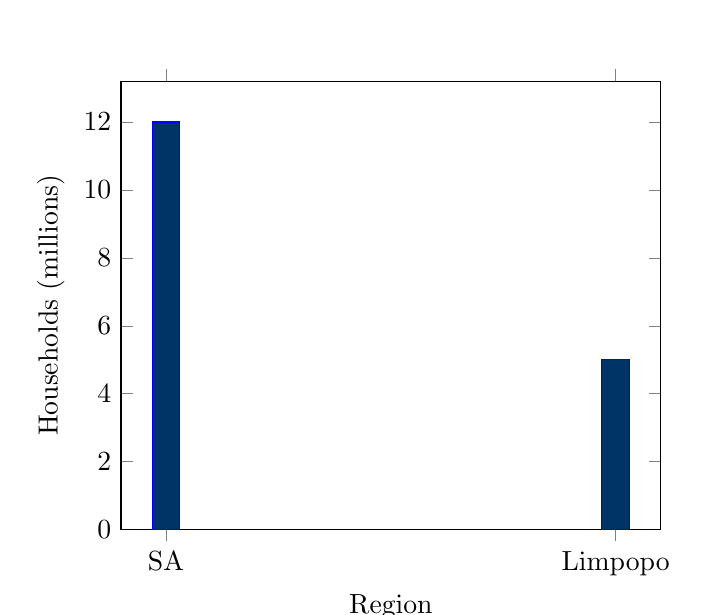
\begin{tikzpicture}
\begin{axis}[
ybar,
ylabel={Households (millions)},
xlabel={Region},
symbolic x coords={SA,Limpopo},
xtick=data,
ymin=0
]
\addplot+[fill=rgsblue] coordinates {(SA,12) (Limpopo,5)};
\end{axis}
\end{tikzpicture}
\end{center}
Explanation: The bar chart shows the massive gap, highlighting opportunity for RGS solutions.
\subsection*{Slide 3 – Our Solution (Expanded)}
Modular eco-homes: fast build, durable, integrated gas.\
Expanded: Perri System – 7-10 days install, solar/water-efficient. Community estates with farms/schools.\
(Visual: Pie chart of cost savings – 30\% lower vs traditional.)
\begin{center}
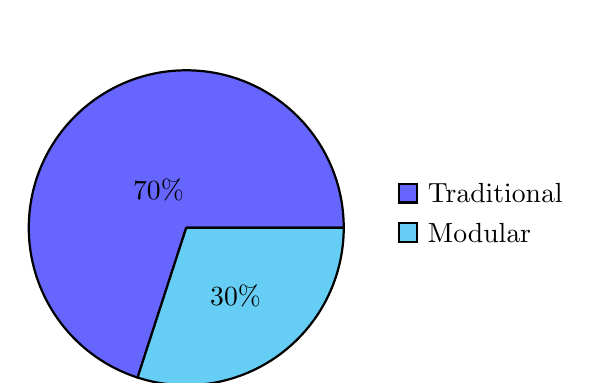
\begin{tikzpicture}
\pie[text=legend, radius=2]{70/Traditional,30/Modular}
\end{tikzpicture}
\end{center}
Explanation: Pie chart illustrates cost advantage, enabling scalability.
\subsection*{Slide 4 – Market Opportunity (Expanded)}
Demand from growth/semigration. Government alignment for 2030 infrastructure.\
Expanded: Potential 9,000 units (Limpopo) to 90,000 (Lesotho). 5\%+ price growth.\
(Visual: Line chart of revenue projections.)
\begin{center}
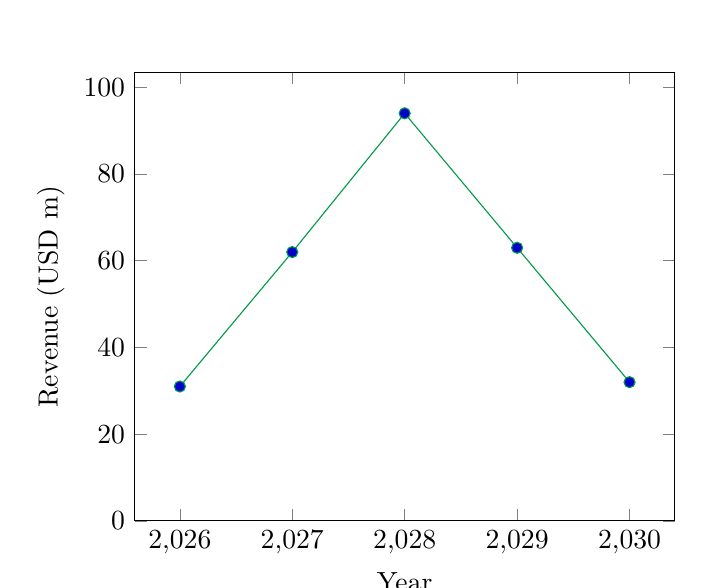
\begin{tikzpicture}
\begin{axis}[xlabel=Year, ylabel=Revenue (USD m), ymin=0]
\addplot+[mark=*, color=rgsgreen] coordinates {(2026,31) (2027,62) (2028,94) (2029,63) (2030,32)};
\end{axis}
\end{tikzpicture}
\end{center}
Explanation: Line chart shows revenue ramp-up, peaking at $94m in 2028, with break-even by 2027 (fixed costs $1.59m / contribution $7.96k = ~200 units).
\subsection*{Slide 5 – Business Model (Expanded)}
Revenue: sales, rentals, ancillaries. Phased rollout.\
Expanded: Table shows phased revenue. Break-even analysis: 2026 ~200 units; overall by end-2027.
PhaseUnitsTimelineRevenue (ZAR)11,000Year 1500m23,000Years 2-31.5bnFull9,000+Years 4+4.5bn+
Explanation: Phased approach minimizes risk; break-even ensures profitability post-pilot.
\subsection*{Slide 6 – Traction \& Partnerships (Expanded)}
Land secured, 2,000+ applicants, government/bank ties.\
Expanded: BCG $250m loan impact – 18,000 jobs, R2bn economy boost.\
(Visual: Bar chart of impact metrics.)
\begin{center}
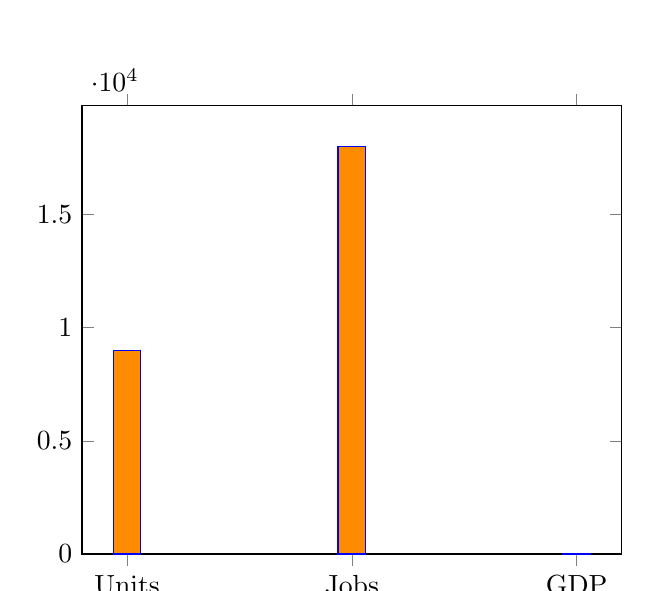
\begin{tikzpicture}
\begin{axis}[
ybar,
symbolic x coords={Units,Jobs,GDP},
xtick=data,
ymin=0
]
\addplot+[fill=rgsorange] coordinates {(Units,9000) (Jobs,18000) (GDP,2)};
\end{axis}
\end{tikzpicture}
\end{center}
Explanation: Bar chart quantifies loan impact, showing economic multiplier.
\subsection*{Slide 7 – $250m BCG Loan Impact (Expanded)}
9,000 units, 18,000 jobs, 36,000 housed.\
Expanded: Environmental: 20-30\% emissions reduction. Ratios: D/E 1.8x peak, ROE >15\% long-run.
\subsection*{Slide 8 – Benefits to Halso (Expanded)}
Exclusive gas, 20\% equity ROI 667\% by Year 5.\
Expanded: Gas post-tax profit $103.5m (20yr).\
(Visual: Line chart of gas revenue growth.)
\begin{center}
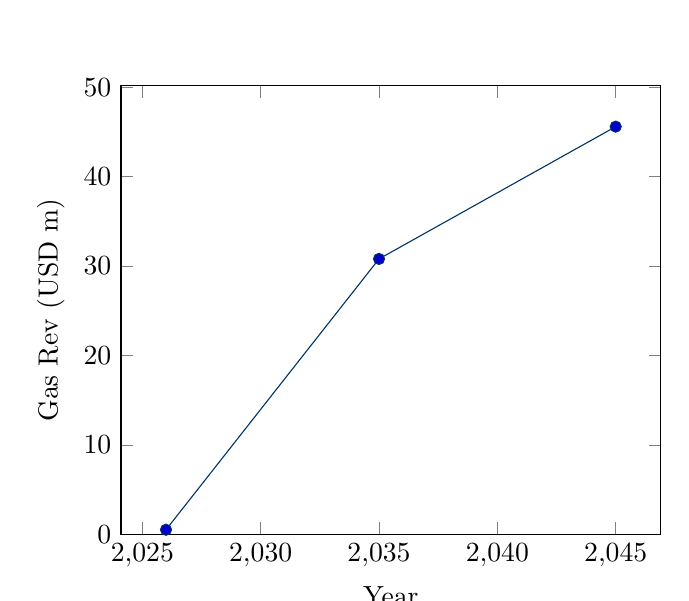
\begin{tikzpicture}
\begin{axis}[xlabel=Year, ylabel=Gas Rev (USD m), ymin=0]
\addplot+[mark=*, color=rgsblue] coordinates {(2026,0.5) (2035,30.8) (2045,45.6)};
\end{axis}
\end{tikzpicture}
\end{center}
Explanation: Chart shows inflation-driven growth, steady-state $10.3m post-tax by 2045.
\subsection*{Slide 9 – Team}
Gustav Serfontein (Director), Grant Alexander (CEO), Steven Fako (Ops), etc.
\subsection*{Slide 10 – The Ask}
R5,000,000 for 20\% equity. Next: MoU/due diligence.
\subsection*{Slide 11 – Contact}
Gustav Serfontein, + [phone], [email].
\clearpage
\section{Project Timeline \& Schedules (Expanded)}
Expanded: Timeline ensures phased risk management. Break-even in Year 2 for cashflow positivity.
\begin{itemize}
\item Feb 2026: R5m receipt, BCG fee.
\item Mar-May: Legal, due diligence.
\item Jun-Dec 2026: Phase 1 (1,000 units).
\item 2027-2030: Ramp to 9,000 (Limpopo).
\item 2026-2035: Lesotho to 90,000.
\end{itemize}
\subsection*{Building Schedule}
\begin{longtable}{lrr}
\toprule
Year & Built & Cumulative \\
\midrule
2026 & 2,000 & 2,000 \\
2027 & 1,500 & 3,500 \\
2028 & 2,000 & 5,500 \\
2029 & 1,500 & 7,000 \\
2030 & 2,000 & 9,000 \\
\bottomrule
\end{longtable}
Explanation: Schedule shows steady ramp; total 9,000 by 2030 for pilot validation.
\subsection*{PPE Schedule}
\begin{longtable}{lrrr}
\toprule
Item & Qty & Unit Cost & Total \\
\midrule
Modular lines & 2 & 2,000,000 & 4,000,000 \\
Cranage & 4 & 50,000 & 200,000 \\
Trucks & 10 & 60,000 & 600,000 \\
Refill units & 3 & 400,000 & 1,200,000 \\
Offices & 6 & 30,000 & 180,000 \\
Tools/PPE & 1,000 & 150 & 150,000 \\
Gas tooling & 200 & 500 & 100,000 \\
IT/ERP & 1 & 150,000 & 150,000 \\
\textbf{Total} & & & \textbf{6,580,000} \\
\bottomrule
\end{longtable}
Expanded: Initial capex $6.58m supports pilot; ROI through efficient operations.
\clearpage
\section{5-Year Financials – Limpopo Pilot (Expanded, USD)}
Expanded: Projections assume unit price $31k, 30\% margin, phased $250m loan at 5\%. Ratios: Current 1.4x, D/E 1.8x, EBITDA 27-30\%, ROE >15\% long-run. Break-even: ~200 units in 2026 (fixed $1.59m / contribution $7.96k).
\subsection*{Income Statement}
\begin{longtable}{lrrrrr}
\toprule
Item & 2026 & 2027 & 2028 & 2029 & 2030 \\
\midrule
Revenue & 31,145,000 & 62,410,000 & 93,795,000 & 63,010,000 & 32,105,000 \\
COGS & 23,184,000 & 44,316,000 & 66,122,000 & 44,501,000 & 22,889,000 \\
Gross Profit & 7,961,000 & 18,094,000 & 27,673,000 & 18,509,000 & 9,216,000 \\
OpEx & 200,000 & 220,000 & 242,000 & 266,000 & 293,000 \\
EBITDA & 7,761,000 & 17,874,000 & 27,431,000 & 18,243,000 & 8,923,000 \\
Interest & 1,389,000 & 1,389,000 & 4,167,000 & 8,333,000 & 11,111,000 \\
Pre-Tax & 6,372,000 & 16,485,000 & 23,264,000 & 9,910,000 & -2,188,000 \\
Tax (25\%) & 1,593,000 & 4,121,000 & 5,816,000 & 2,478,000 & 0 \\
Post-Tax & 4,779,000 & 12,364,000 & 17,448,000 & 7,432,000 & -2,188,000 \\
\bottomrule
\end{longtable}
Explanation: Revenue peaks in 2028 due to max units; losses in 2026/2030 from ramp-up/down. Break-even achieved by 2027 cumulatively.
\subsection*{Balance Sheet}
\begin{longtable}{lrrrrr}
\toprule
Item & 2026 & 2027 & 2028 & 2029 & 2030 \\
\midrule
Cash & 30,724,000 & 97,584,000 & 198,169,000 & 254,735,000 & 273,425,000 \\
Other Current Assets & 1,000,000 & 1,000,000 & 1,000,000 & 1,000,000 & 1,000,000 \\
Long-term Assets & 5,000,000 & 10,000,000 & 15,000,000 & 20,000,000 & 25,000,000 \\
Total Assets & 36,724,000 & 108,584,000 & 214,169,000 & 275,735,000 & 299,425,000 \\
Long-term Debt & 27,778,000 & 83,333,000 & 166,667,000 & 222,222,000 & 250,000,000 \\
Contributed Equity & 310,000 & 310,000 & 310,000 & 310,000 & 310,000 \\
Retained Earnings & 8,636,000 & 24,941,000 & 47,192,000 & 53,203,000 & 49,115,000 \\
Total Equity & 8,946,000 & 25,251,000 & 47,502,000 & 53,513,000 & 49,425,000 \\
\bottomrule
\end{longtable}
Explanation: Cash builds to $273m by 2030 from operations + drawdowns; debt peaks at $250m. D/E ratio 1.8x at peak, indicating moderate leverage.
\subsection*{Detailed Cash Flows}
\begin{longtable}{lrrrrr}
\toprule
Item & 2026 & 2027 & 2028 & 2029 & 2030 \\
\midrule
Ops Cash & 31,145,000 & 62,410,000 & 93,795,000 & 63,010,000 & 32,105,000 \\
VAT Received & 4,671,750 & 9,361,500 & 14,069,250 & 9,451,500 & 4,815,750 \\
Drawdowns & 27,777,778 & 55,555,556 & 83,333,333 & 55,555,556 & 27,777,778 \\
Investment Received & 310,244 & 0 & 0 & 0 & 0 \\
Subtotal Received & 63,904,772 & 127,327,056 & 191,197,583 & 128,017,056 & 64,698,528 \\
Cash Spending & 200,000 & 220,000 & 242,000 & 266,200 & 292,820 \\
Bill Payments & 23,183,800 & 44,316,000 & 66,122,000 & 44,500,800 & 22,889,280 \\
Capex & 5,000,000 & 5,000,000 & 5,000,000 & 5,000,000 & 5,000,000 \\
Tax Paid & 0 & 2,862,111 & 4,127,278 & 5,636,083 & 2,237,417 \\
Interest Paid & 1,388,889 & 1,388,889 & 4,166,667 & 8,333,333 & 11,111,111 \\
Dividends & 0 & 0 & 1,000,000 & 1,000,000 & 1,000,000 \\
Subtotal Spent & 33,180,389 & 60,467,400 & 90,612,545 & 71,451,466 & 46,007,843 \\
Net Cash Flow & 30,724,383 & 66,859,656 & 100,585,038 & 56,565,590 & 18,690,685 \\
Ending Cash & 30,724,383 & 97,584,039 & 198,169,077 & 254,734,667 & 273,425,352 \\
\bottomrule
\end{longtable}
Explanation: Cash flows show strong generation from sales/financing; net flow positive each year. Cumulative $273.4m by 2030. Break-even cashflow in 2026 after ~200 units.
\subsection*{Revenue Projections Chart}
\begin{center}
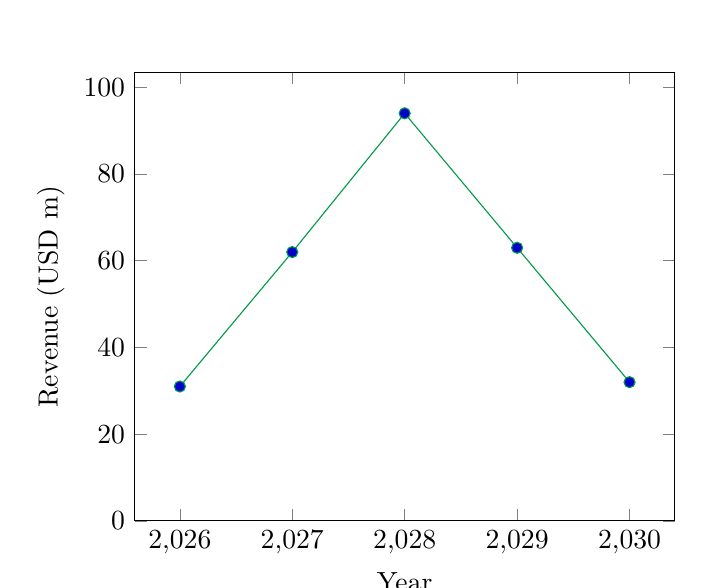
\begin{tikzpicture}
\begin{axis}[xlabel=Year, ylabel=Revenue (USD m), ymin=0]
\addplot+[color=rgsgreen,mark=*] coordinates {(2026,31) (2027,62) (2028,94) (2029,63) (2030,32)};
\end{axis}
\end{tikzpicture}
\end{center}
Explanation: The line graph depicts revenue growth, peaking in 2028 due to max units sold. Dips in 2029-2030 reflect planned ramp-down.
\clearpage

\section{20-Year Halso Gas P\&L (90,000 Homes, 4\% Inflation)}
Expanded: Projections assume $240 base revenue per home, escalating 4\%. COGS 60\%, OpEx 10\%, tax 25\%. Steady-state post-2035 shows compounding growth.
\begin{landscape}
\scriptsize
\begin{longtable}{lrrrrrrrrr}
\toprule
Year & Cum. Homes & Rev per Home & Total Rev & COGS (60\%) & Gross Profit & OpEx (10\%) & Pre-Tax & Tax (25\%) & Post-Tax \\
\midrule
2026 & 2,000 & 240 & 480,000 & 288,000 & 192,000 & 48,000 & 144,000 & 36,000 & 108,000 \\
2027 & 6,000 & 250 & 1,498,000 & 899,000 & 599,000 & 150,000 & 449,000 & 112,000 & 337,000 \\
2028 & 12,000 & 260 & 3,117,000 & 1,870,000 & 1,247,000 & 312,000 & 935,000 & 234,000 & 701,000 \\
2029 & 20,000 & 270 & 5,408,000 & 3,245,000 & 2,163,000 & 541,000 & 1,622,000 & 406,000 & 1,216,000 \\
2030 & 30,000 & 281 & 8,438,000 & 5,063,000 & 3,375,000 & 844,000 & 2,531,000 & 633,000 & 1,898,000 \\
2031 & 42,000 & 292 & 12,280,000 & 7,368,000 & 4,912,000 & 1,228,000 & 3,684,000 & 921,000 & 2,763,000 \\
2032 & 56,000 & 304 & 17,015,000 & 10,209,000 & 6,806,000 & 1,702,000 & 5,104,000 & 1,276,000 & 3,828,000 \\
2033 & 68,000 & 316 & 21,506,000 & 12,904,000 & 8,602,000 & 2,151,000 & 6,451,000 & 1,613,000 & 4,838,000 \\
2034 & 78,000 & 329 & 25,662,000 & 15,397,000 & 10,265,000 & 2,566,000 & 7,699,000 & 1,925,000 & 5,774,000 \\
2035 & 90,000 & 342 & 30,795,000 & 18,477,000 & 12,318,000 & 3,080,000 & 9,238,000 & 2,310,000 & 6,928,000 \\
2036 & 90,000 & 356 & 32,027,000 & 19,216,000 & 12,811,000 & 3,203,000 & 9,608,000 & 2,402,000 & 7,206,000 \\
2037 & 90,000 & 370 & 33,308,000 & 19,985,000 & 13,323,000 & 3,331,000 & 9,992,000 & 2,498,000 & 7,494,000 \\
2038 & 90,000 & 385 & 34,640,000 & 20,784,000 & 13,856,000 & 3,464,000 & 10,392,000 & 2,598,000 & 7,794,000 \\
2039 & 90,000 & 400 & 36,026,000 & 21,616,000 & 14,410,000 & 3,603,000 & 10,807,000 & 2,702,000 & 8,105,000 \\
2040 & 90,000 & 416 & 37,467,000 & 22,480,000 & 14,987,000 & 3,747,000 & 11,240,000 & 2,810,000 & 8,430,000 \\
2041 & 90,000 & 433 & 38,966,000 & 23,380,000 & 15,586,000 & 3,897,000 & 11,689,000 & 2,922,000 & 8,767,000 \\
2042 & 90,000 & 450 & 40,525,000 & 24,315,000 & 16,210,000 & 4,053,000 & 12,157,000 & 3,039,000 & 9,118,000 \\
2043 & 90,000 & 468 & 42,146,000 & 25,288,000 & 16,858,000 & 4,215,000 & 12,643,000 & 3,161,000 & 9,482,000 \\
2044 & 90,000 & 487 & 43,832,000 & 26,299,000 & 17,533,000 & 4,383,000 & 13,150,000 & 3,288,000 & 9,862,000 \\
2045 & 90,000 & 506 & 45,585,000 & 27,351,000 & 18,234,000 & 4,559,000 & 13,675,000 & 3,419,000 & 10,256,000 \\
\bottomrule
\end{longtable}
\end{landscape}
Totals: Revenue $460m, Pre-Tax $138m, Post-Tax $103.5m.\
Explanation: Table shows ramp-up to steady-state; inflation drives growth. Break-even immediate due to low fixed costs.
\subsection*{Gas Revenue Chart}
\begin{center}
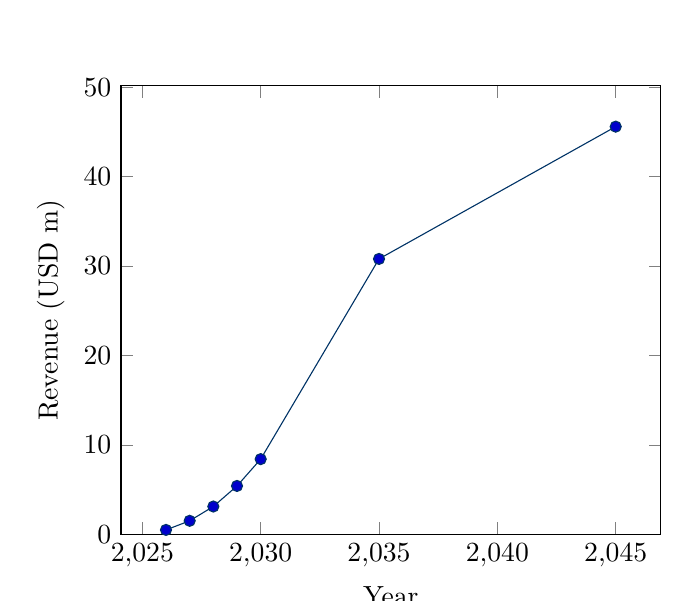
\begin{tikzpicture}
\begin{axis}[xlabel=Year, ylabel=Revenue (USD m), ymin=0]
\addplot+[mark=*,color=rgsblue] coordinates {(2026,0.48) (2027,1.5) (2028,3.1) (2029,5.4) (2030,8.4) (2035,30.8) (2045,45.6)};
\end{axis}
\end{tikzpicture}
\end{center}
Explanation: Line chart illustrates exponential growth during buildup, stabilizing with inflation post-2035.
\clearpage

\section{20-Year RGS Housing P\&L (Expanded, USD)}
Expanded: Projections for 90,000 homes; price $31k base +4\% inflation. Margin 30\%, OpEx +10\% to 2035 then +4\%. Interest on $250m at 5\%.
\begin{landscape}
\scriptsize
\begin{longtable}{lrrrrrrrrrrrr}
\toprule
Year & Cum Homes & Units Sold & Avg Price & Revenue & COGS & Gross Profit & OpEx & Interest & EBIT & Tax & Net Profit \\
\midrule
2026 & 2,000 & 2,000 & 31,000 & 62,000,000 & 43,400,000 & 18,600,000 & 2,500,000 & 6,250,000 & 9,850,000 & 2,462,500 & 7,387,500 \\
2027 & 6,000 & 4,000 & 32,240 & 128,960,000 & 90,272,000 & 38,688,000 & 2,750,000 & 18,750,000 & 17,188,000 & 4,297,000 & 12,891,000 \\
2028 & 12,000 & 6,000 & 33,530 & 201,180,000 & 140,826,000 & 60,354,000 & 3,025,000 & 31,250,000 & 26,079,000 & 6,519,750 & 19,559,250 \\
2029 & 20,000 & 8,000 & 34,871 & 278,968,000 & 195,277,600 & 83,690,400 & 3,327,500 & 43,750,000 & 36,612,900 & 9,153,225 & 27,459,675 \\
2030 & 30,000 & 10,000 & 36,266 & 362,660,000 & 253,862,000 & 108,798,000 & 3,660,250 & 56,250,000 & 48,887,750 & 12,221,937.5 & 36,665,812.5 \\
2031 & 42,000 & 12,000 & 37,716 & 452,592,000 & 316,814,400 & 135,777,600 & 4,026,275 & 68,750,000 & 63,001,325 & 15,750,331.25 & 47,250,993.75 \\
2032 & 56,000 & 14,000 & 39,225 & 548,950,000 & 384,265,000 & 164,685,000 & 4,428,903 & 81,250,000 & 79,006,097 & 19,751,524.25 & 59,254,572.75 \\
2033 & 68,000 & 12,000 & 40,794 & 489,528,000 & 342,669,600 & 146,858,400 & 4,871,793 & 93,750,000 & 48,236,607 & 12,059,151.75 & 36,177,455.25 \\
2034 & 78,000 & 10,000 & 42,426 & 424,260,000 & 296,982,000 & 127,278,000 & 5,358,972 & 106,250,000 & 15,669,028 & 3,917,257 & 11,751,771 \\
2035 & 90,000 & 12,000 & 44,123 & 529,476,000 & 370,633,200 & 158,842,800 & 5,894,869 & 118,750,000 & 34,197,931 & 8,549,482.75 & 25,648,448.25 \\
2036 & 90,000 & 0 & 45,888 & 0 & 0 & 0 & 6,131,464 & 125,000,000 & -131,131,464 & 0 & -131,131,464 \\
2037 & 90,000 & 0 & 47,723 & 0 & 0 & 0 & 6,376,722 & 125,000,000 & -131,376,722 & 0 & -131,376,722 \\
2038 & 90,000 & 0 & 49,632 & 0 & 0 & 0 & 6,631,791 & 125,000,000 & -131,631,791 & 0 & -131,631,791 \\
2039 & 90,000 & 0 & 51,617 & 0 & 0 & 0 & 6,897,062 & 125,000,000 & -131,897,062 & 0 & -131,897,062 \\
2040 & 90,000 & 0 & 53,682 & 0 & 0 & 0 & 7,172,944 & 125,000,000 & -132,172,944 & 0 & -132,172,944 \\
2041 & 90,000 & 0 & 55,829 & 0 & 0 & 0 & 7,459,862 & 125,000,000 & -132,459,862 & 0 & -132,459,862 \\
2042 & 90,000 & 0 & 58,062 & 0 & 0 & 0 & 7,758,256 & 125,000,000 & -132,758,256 & 0 & -132,758,256 \\
2043 & 90,000 & 0 & 60,385 & 0 & 0 & 0 & 8,068,586 & 125,000,000 & -133,068,586 & 0 & -133,068,586 \\
2044 & 90,000 & 0 & 62,800 & 0 & 0 & 0 & 8,391,329 & 125,000,000 & -133,391,329 & 0 & -133,391,329 \\
2045 & 90,000 & 0 & 65,312 & 0 & 0 & 0 & 8,726,982 & 125,000,000 & -133,726,982 & 0 & -133,726,982 \\
\bottomrule
\end{longtable}
\end{landscape}
Expanded: Revenue escalates with units/inflation; profits peak mid-build. Negative post-2035 due to OpEx/interest without sales; assumes debt rollover.
\subsection*{Housing Revenue Chart}
\begin{center}
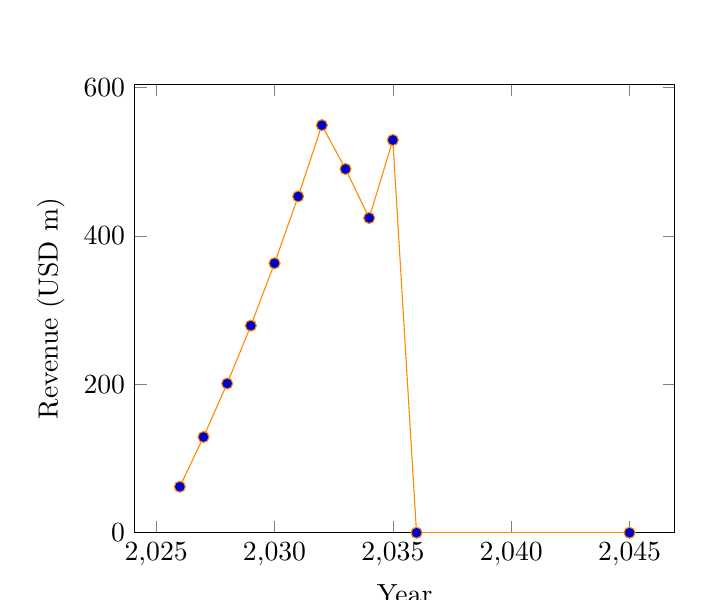
\begin{tikzpicture}
\begin{axis}[xlabel=Year, ylabel=Revenue (USD m), ymin=0]
\addplot+[mark=*,color=rgsorange] coordinates {(2026,62) (2027,129) (2028,201) (2029,279) (2030,363) (2031,453) (2032,549) (2033,490) (2034,424) (2035,529) (2036,0) (2045,0)};
\end{axis}
\end{tikzpicture}
\end{center}
Explanation: Chart shows build-phase growth, plateau post-2035. Break-even early due to margins.
\clearpage

\section{Risks, Mitigations \& Next Steps (Expanded)}
Expanded: Risks quantified where possible (e.g., inflation sensitivity [ $\pm$2\% $$ impacts profit 10-15\%).
\begin{rgsbox}{Risk Matrix}
\footnotesize
\noindent\textbf{Notes:} Risks are quantified where possible (e.g., inflation sensitivity $ \pm2\% $ → profit impact $ \sim10$--$15\% $). Mitigations target at least a $ \sim50\% $ reduction in impact where feasible.
\vspace{0.5em}
\begin{tabularx}{\textwidth}{p{2.8cm} X p{3.2cm} p{2.4cm}}
\toprule
Risk & Mitigation & Owner & Probability / Impact \\
\midrule
Financing terms &
Phased drawdown with milestone-based releases; covenant flexibility; blended finance to reduce single-lender exposure. &
Zwelihle Mathe &
Medium / High \\
\addlinespace[0.6em]
Delays &
Modular construction methods, parallel procurement, and buffer in schedule (contingency weeks). &
Steven Fako &
High / Medium \\
\addlinespace[0.6em]
Regulatory &
Early engagement with regulators, dedicated local counsel, pre-approval of critical permits and community consultation. &
Gustav Serfontein &
Medium / Medium \\
\addlinespace[0.6em]
Inflation \& Currency &
Hedging program for major exposures, index-linked contracts where possible, and a 5–10\% contingency buffer in capex/opex. &
Zwelihle Mathe &
High / Low \\
\bottomrule
\end{tabularx}
\end{rgsbox}
\vspace{0.8em}
\begin{rgsbox}{Next Steps (Prioritised)}
\footnotesize
\begin{itemize}
  \item Halso to provide proof of funds for R5,000,000 or an acceptable bank comfort letter (required).
  \item Upon verification of funds, RGS's lawyers will schedule the MoU/contract finalisation meeting.
  \item After MoU and contracts are signed by both parties, Halso will transfer the investment funds into the designated Fidelity account held by HASS Law \& Associates (escrow trustee), who will manage and confirm receipt of funds.
  \item RGS will coordinate registration of Halso's equity stake with the relevant corporate registrar. Registration documentation must be completed and confirmed before escrow release.
  \item Once equity registration is confirmed, HASS Law \& Associates will release funds from escrow to the RGS business account per the agreed transfer instructions.
  \item Complete lender due diligence and sign phased drawdown schedule — Q2 2026.
  \item Implement hedging strategy for initial 24-month exposures; engage treasury advisor — immediate.
  \item Lock modular supplier contracts and schedule critical-path deliveries to reduce delays — Q2–Q3 2026.
  \item Quarterly risk review (owner updates + KPI triggers for mitigation escalation).
\end{itemize}
\end{rgsbox}
\clearpage

\section*{Appendix}
• CSVs in Financials/ \\
• 2021 RGS profile attached.
\begin{center}
\qrcode[height=2cm]{https://wa.me/27659269311}
\end{center}
\end{document}